\documentclass[11pt]{amsart}
%prepared in AMSLaTeX, under LaTeX2e
\addtolength{\oddsidemargin}{-.9in} 
\addtolength{\evensidemargin}{-.9in}
\addtolength{\topmargin}{-.9in}
\addtolength{\textwidth}{1.5in}
\addtolength{\textheight}{1.5in}

\renewcommand{\baselinestretch}{1.02}

\usepackage{verbatim} % for "comment" environment

\usepackage{palatino}

\usepackage[final]{graphicx}

\usepackage{tikz}
\usetikzlibrary{positioning}

\usepackage{enumitem,xspace,fancyvrb}

\newtheorem*{thm}{Theorem}
\newtheorem*{defn}{Definition}
\newtheorem*{example}{Example}
\newtheorem*{problem}{Problem}
\newtheorem*{remark}{Remark}

\DefineVerbatimEnvironment{mVerb}{Verbatim}{numbersep=2mm,frame=lines,framerule=0.1mm,framesep=2mm,xleftmargin=4mm,fontsize=\footnotesize}

% macros
\usepackage{amssymb,amsmath,bbm}
\newcommand{\bA}{\mathbf{A}}
\newcommand{\bB}{\mathbf{B}}
\newcommand{\bE}{\mathbf{E}}
\newcommand{\bF}{\mathbf{F}}
\newcommand{\bJ}{\mathbf{J}}

\newcommand{\bb}{\mathbf{b}}
\newcommand{\bi}{\mathbf{i}}
\newcommand{\bj}{\mathbf{j}}
\newcommand{\bk}{\mathbf{k}}
\newcommand{\br}{\mathbf{r}}
\newcommand{\bu}{\mathbf{u}}
\newcommand{\bv}{\mathbf{v}}
\newcommand{\bw}{\mathbf{w}}
\newcommand{\bx}{\mathbf{x}}

\newcommand{\ppr}[1]{\frac{\partial #1}{\partial r}}
\newcommand{\ppt}[1]{\frac{\partial #1}{\partial t}}
\newcommand{\ppx}[1]{\frac{\partial #1}{\partial x}}
\newcommand{\ppy}[1]{\frac{\partial #1}{\partial y}}
\newcommand{\ppz}[1]{\frac{\partial #1}{\partial z}}

\newcommand{\Div}{\ensuremath{\nabla\cdot}}
\newcommand{\Curl}{\ensuremath{\nabla\times}}

\newcommand{\eps}{\epsilon}
\newcommand{\grad}{\nabla}
\newcommand{\ip}[2]{\ensuremath{\left<#1,#2\right>}}
\newcommand{\lam}{\lambda}
\newcommand{\lap}{\triangle}

\newcommand{\RR}{\mathbb{R}}
\newcommand{\ZZ}{\mathbb{Z}}
\newcommand{\prob}[1]{\bigskip\noindent\textbf{#1.}\quad }

\newcommand{\Matlab}{\textsc{Matlab}\xspace}

\newcommand{\ds}{\displaystyle}

\begin{document}
\scriptsize \hfill \today

\Large
\bigskip
\centerline{\textbf{A family of exact solutions to the 1D $p$-Laplacian obstacle problem}}
\bigskip

\normalsize

\thispagestyle{empty}

For the purposes of building a nonlinear variational inequality verification case we will construct exact solutions to the one-dimensional case of the \emph{$p$-Laplacian obstacle problem}.  Over an open set $\Omega\subset \RR^d$, for $p>1$, $f \in L^1(\Omega)$, and $\psi \in W^{1,p}(\Omega)$, recall that the problem is to find $u(x) \ge \psi(x)$ satisfying
\begin{equation}
-\Div\left(|\grad u(x)|^{p-2} \grad u(x)\right) = f(x) \qquad \text{on the set where } u(x) > \psi(x). \label{plap}
\end{equation}

The weak form of this problem is well-posed with Dirichlet boundary conditions, and in particular there is a unique solution $u \in \mathcal{K}=\{v \ge \psi\} \subset W_0^{1,p}(\Omega)$ \cite{KinderlehrerStampacchia1980}.  Equivalently, the coercive functional $J[u] = \int_\Omega \frac{1}{p} |\grad u|^p - f u$ has a unique minimum over $\mathcal{K}$, a closed and convex subset.  Observe that if $p=2$ then the operator is the ordinary Laplacian.  If $1<p<2$ then $D=|\grad u|^{p-2}>0$ is unbounded as $|\grad u| \to 0$ (\emph{fast diffusion}), while if $p>2$ then $D\to 0$ as $|\grad u| \to 0$ (\emph{degenerate diffusion}).  The degenerate case violates uniform ellipticity, despite coercivity.

We will solve a one-dimensional case of \eqref{plap}, with
\begin{equation}
f(x) = \begin{cases} \alpha, & |x| < 1 \\ -\alpha, & |x| > 1\end{cases} \qquad \text{and} \qquad \psi(x) = - \beta |x| \label{data}
\end{equation}
on the interval $\Omega = (-3,3) \subset \RR^1$, for $\alpha > 0$ and $\beta \ge 0$.
% FIXME  I think the cases where \beta < 0$ are fine too, though eventually the free boundary will be outside $(-3,3)$
That is, we seek $u(x) \ge -\beta |x|$ so that
\begin{equation}
-\left(|u'(x)|^{p-2} u'(x)\right)' = \alpha \left(\mathbbm{1}_{(-1,1)}(x) - \mathbbm{1}_{(-3,-1)\cup(1,3)}(x)\right).  \label{concrete}
\end{equation}

By symmetry and well-posedness, $u(x)$ is an even function and $u'(0)=0$.  Restricting attention to $x\ge 0$, we will see that $u'(x)\le 0$ for $x\le 2$.  Integrating \eqref{concrete} once gives
    $$\left(-u'(x)\right)^{p-1} = \int_0^x f(t)\,dt = \begin{cases} \alpha x, & 0 \le x \le 1 \\ \alpha (2 - x), & x \ge 1\end{cases}$$
The function on the right is continuous.  Solving for $u'(x)$ by raising to the $(p-1)^{-1} = q-1$ power, where $\frac{1}{p} + \frac{1}{q} = 1$ defines the dual exponent $q>1$, gives
    $$u'(x) = \begin{cases} - \alpha^{q-1} x^{q-1}, & 0 \le x \le 1 \\ -\alpha^{q-1} (2 - x)^{q-1}, & x \ge 1\end{cases}$$
Note that $u''(x) < 0$ (concave) for $0 < x < 1$ and $u''(x)>0$ (convex) for $x>1$.

Integrating again, and recalling that $u(x)$ has even symmetry, for some $u(0)$ to be determined, we have
\begin{align*}
u(x) &= \begin{cases} u(0) - \frac{\alpha^{q-1}}{q} |x|^q, & |x| \le 1 \\
                      u(0) - \frac{\alpha^{q-1}}{q} -\alpha^{q-1} \int_1^{|x|} (2 - y)^{q-1}\,dy, & |x| \ge 1\end{cases} \\
     &= \begin{cases} u(0) - \frac{\alpha^{q-1}}{q} |x|^q, & |x| \le 1 \\
                      u(0) + \frac{\alpha^{q-1}}{q} \left( (2 - |x|)^q - 2 \right), & |x| \ge 1\end{cases}
\end{align*}

Now, where is the free boundary?  It must occur at $x=\xi>0$ where simultaneously $u(\xi)=-\beta \xi$ and $u'(\xi)=-\beta\le 0$.  However, $u'(2)=0$, which reflects the symmetry that the integral of $f(x)$ on $[0,1]$ is cancelled by its integral on $[1,2]$.  Furthermore $u'(x)<0$ for $0<x<2$ and $u'(x)$ is minimum at $x=1$, with $u'(1) = -\alpha^{q-1}$.  By a convexity/concavity argument, existence of the free boundary requires $\alpha^{q-1}/q>\beta$, which implies $\beta^{p-1}/\alpha < 1$ (see below).  Then, because $\beta \ge 0$, tangency implies that the free boundary is at some $1 < \xi \le 2$, and the above calculation is justified.

Thus, given $\alpha>0$ and $0 \le \beta < \alpha^{q-1}/q$, we solve the system $u'(\xi)=-\beta$ and $u(\xi)=-\beta \xi$:
\begin{align*}
-\alpha^{q-1} (2 - \xi)^{q-1} &= -\beta \\
u(0) + \frac{\alpha^{q-1}}{q} \left( (2 - \xi)^q - 2 \right) &= -\beta \xi
\end{align*}
The first equation determines $\xi$ and then the second will yield $u(0)$.  If $\beta=0$ then the free boundary is at $\xi=2$ and thus $u(0) = 2 \alpha^{q-1} / q$.  Generally
\begin{equation}
\boxed{\xi = 2 - \frac{\beta^{p-1}}{\alpha} \qquad \text{and} \qquad u(0) = \frac{\beta^p}{p \alpha} + 2 \left(\frac{\alpha^{q-1}}{q} - \beta\right).} \label{params}
\end{equation}

In conclusion, our exact solution family starts with a choice of $p>1$ and $\alpha>0$ arbitrary.  Let $q>1$ be the dual exponent and choose $\beta \in [0,\alpha^{q-1}/q)$.  Compute $\xi \in (1,2]$ and $u(0)>0$ by \eqref{params}.  Then 
\begin{equation}
\boxed{u(x) = \begin{cases} u(0) - \frac{\alpha^{q-1}}{q} |x|^q, & |x| \le 1 \\
                      u(0) + \frac{\alpha^{q-1}}{q} \left( (2 - |x|)^q - 2 \right), & 1 \le |x| \le \xi \\
                      -\beta |x|, & \xi \le |x| \le 3\end{cases}}  \label{exact}
\end{equation}
This function is in $W^{1,p}(\Omega) \cap W^{2,\infty}(\Omega)$, where $\Omega = (-3,3)$, and specifically it is continuously-differentiable.  It satisfies \eqref{plap} strongly a.e.

The $\beta=0$ case, in which the obstacle $\psi(x)=0$ is flat, implies that the solution has zero gradient at the free boundary ($u'(\xi)=0$).  Note that this implies a loss of uniform ellipticity at the free boundary in the $p>2$ degenerate diffusion cases, which makes the obstacle problem very challenging numerically, so we avoid that difficulty by setting $\beta>0$.

For numerical tests we set parameters $\alpha=1$ and $\beta = 0.2$, and consider powers $p=3/2,2,4$, corresponding to $q=3,2,4/3$ respectively.  (For these $\alpha,\beta$ values, the requirement $\beta < \alpha^{q-1}/q$ is satisfied when $p > 5/4$.)  Numerical and exact solutions for the $p=3/2$ and $p=4$ cases are shown in Figure \ref{fig:solutions}.

\begin{figure}
\mbox{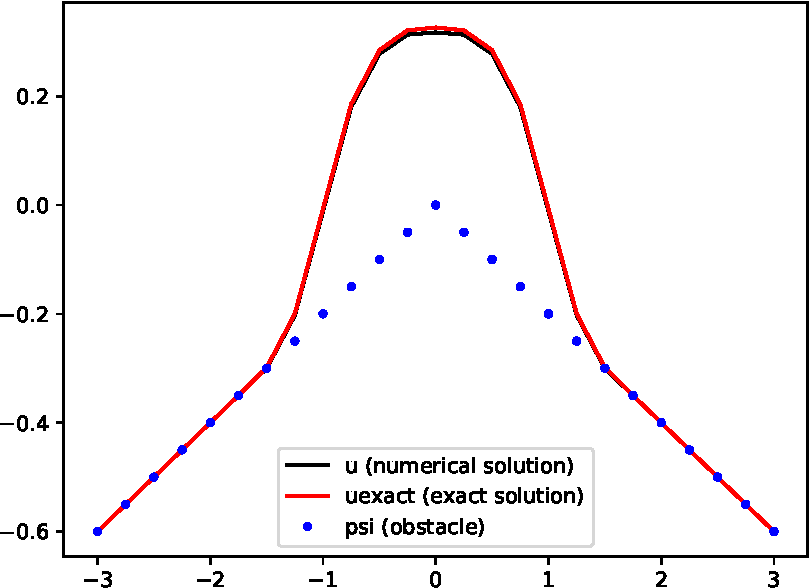
\includegraphics[width=0.45\textwidth]{solution1p5.pdf} \qquad 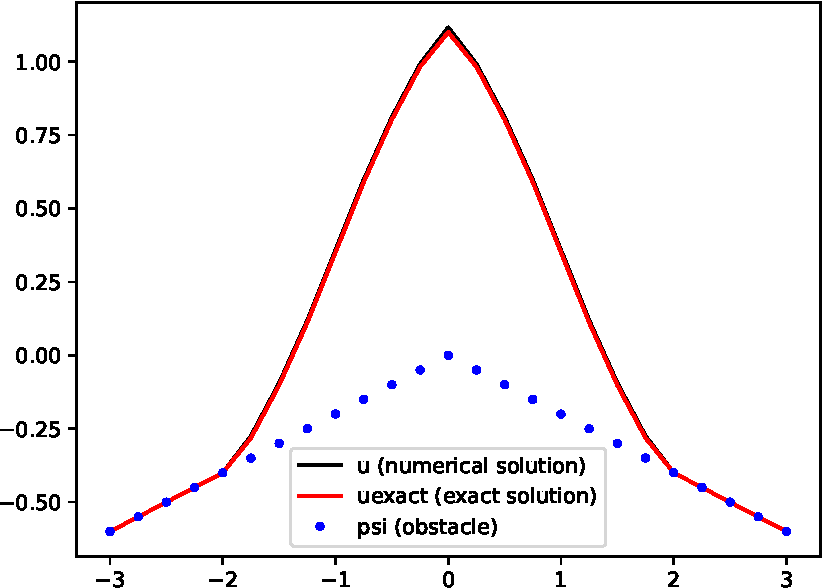
\includegraphics[width=0.45\textwidth]{solution4.pdf}}
\caption{Low-resolution $p$-Laplacian obstacle problem solutions for $\alpha=1$, $\beta=0.2$, and $p=1.5$ (left) or $p=4$ (right).}
\label{fig:solutions}
\end{figure}



\begin{thebibliography}{1}

\bibitem{KinderlehrerStampacchia1980}
{\sc D.~Kinderlehrer and G.~Stampacchia}, {\em An {I}ntroduction to
  {V}ariational {I}nequalities and their {A}pplications}, Academic Press, New
  York, 1980.

\end{thebibliography}
\end{document}
